% !TeX encoding = UTF-8
% !TeX root = ROSCostMapZh-Cn.tex
% !TeX TS-program = xelatex.exe

%https://blog.csdn.net/xmy306538517/article/details/72899667

\section{简介}

过去的几十年里,导航算法变得越来越复杂。
它们处理大量传感器的数据,高精度跟踪障碍物位置和自由空间。
结合正确的路径规划算法,它们可以很熟练地在环境中进行巡航。
然而,很多这类导航算法也遇到同样的问题:算法皆是为了产生无碰撞的自由路径进行有效寻优。

这种算法在许多实际用例或抽象环境下表现很好,如果都是要求从点A走到点B。
对于其他实际用例来说还不是特别好。
像在人口稠密的动态环境中移动的机器人,需要集成更复杂的约束到优化问题中。
从一个点走到另一个点只是一个更大区域的上下文的一部分。
机器人围绕障碍物移动仅是为了避免碰撞是不够的;
机器人必须根据上下文语义的不同区别对待该障碍。
例如,大多数情况,在远离桌子几厘米之外行走是完全没有问题的。
然而,紧贴着人群行走更是不希望发生的。
%我们绝不希望紧密的贴着人驾驶。
%然而,在等价对待所有障碍的成本图中,路径规划者无法选择一条正确的路径。
如果导航算法平等对待所有感知到的障碍物,此时规划器可能无法选择出一条正确的行走路径。


规划路径时,除了尊重他人的个人空间这种场合之外,还有许多其他的场合表明:选择最短的无碰撞路径可能不是最理想的。
若考虑人群中人经常聚集的位置信息,此时应该首选避免可能有障碍的长度更长的路径。
机器人还必须考虑进入有潜在危险区域的场景时的实用情况,例如厨房,虽然是有效的路径,但这些区域应该带有通行代价。
即使对一些简单因素也应该作考虑,比如在走廊的右侧驾驶。
机器人选择走哪条路取决于在大环境提取的额外的上下文信息。

路径规划器使用的环境信息皆存储于一张代价地图上。
在传统的代价图中,所有的数据都存储在一个单元网格中,我们称之为\CJKNhl{单体代价地图} (monolithic costmap)。
单体代价地图由于只需要在一个地方读写代价值,非常简单,是一种很流行的技术。
它的一个结果是代价地图中相当多的代价值被丢弃,使得对地图的周期维护变得越来越困难。

本文中,我们介绍一种将额外上下文信息到代价地图方案,方案采用了一种称之为\CJKNhl{分层代价地图} (layered costmaps) 的新方法。通过使用ROS导航框架作为试点,我们展示分层代价地图在复现以前导航算法的功能的同时,能增加处理更多上下文信息的灵活性。
图\ref{fig:costMap:layers}展示了一种分层代价地图的可能的配置方式。
我们将讨论该算法和数据结构,以及相对以前方法的改进点。
之后,我们将对可以加入到新旧代价地图中的不同层和它们所集成的环境上下文进行检查(以讨论它们对规划的路径的影响)。

\begin{figure}[!htb]
	\centering
	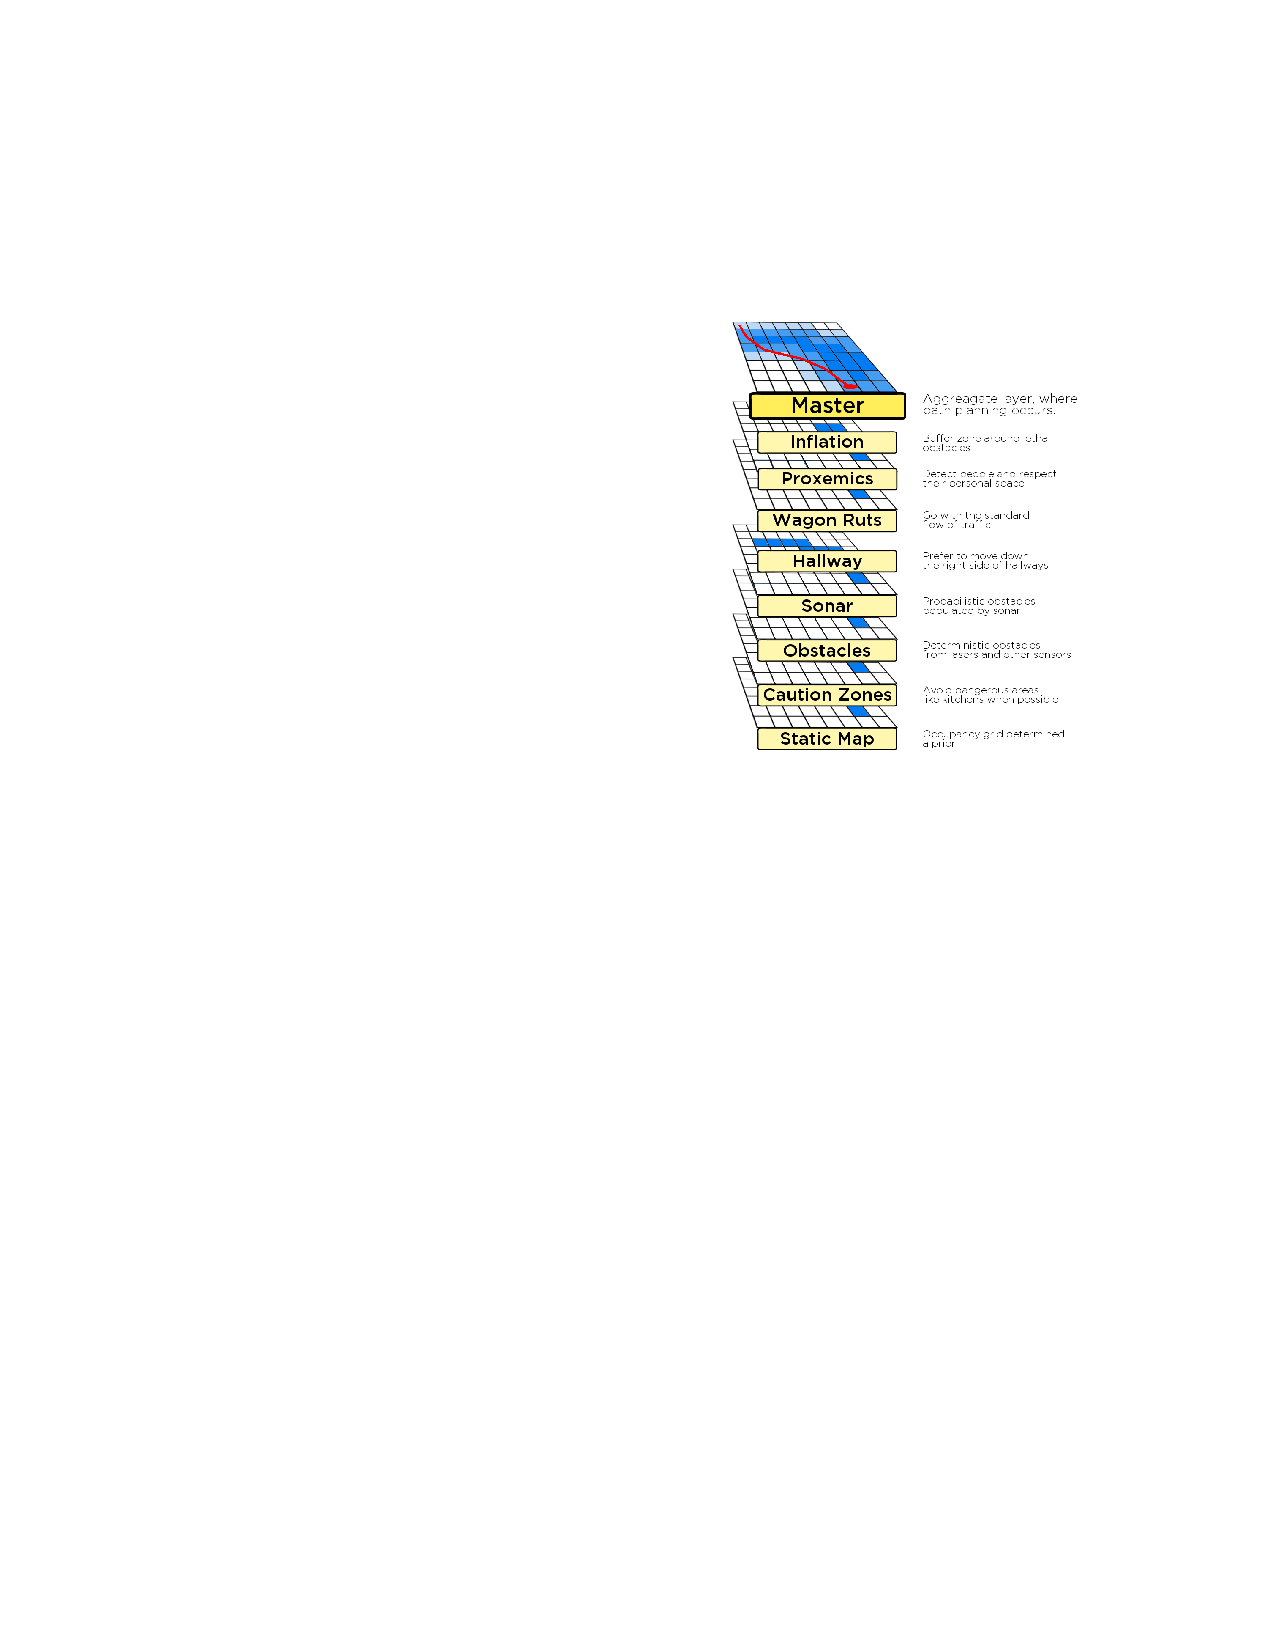
\includegraphics[width=0.45\linewidth]{layeredMaps}
	\caption{一组costmap图层,展示了使用分层costmap方法可实现的不同上下文行为。}
	\label{fig:costMap:layers}
\end{figure}

\section{相关工作}
这项工作的重点是适用于规划路径的地图的网格表示方式。 
20世纪80年代,由Moravec及其合作者在卡内基梅隆大学(CMU)开发的占据网格(occupancy grid)是现代代价地图鼻祖\cite{matthies1988integration,moravec1989sensor}。 
占据网格的语义值很直观:每个单元格的值表示该单元格存在障碍物的概率,因此其更新过程是贝叶斯规则的直接应用。 
Konolige\cite{konolige1997improved}和Thrun\cite{thrun2001learning}改进了概率模型,以便更好地定位障碍物。
基于网格的代价地图表示方法(其中网格值表示的不是概率而是通行代价)被证明是很实用的方法,尤其是当障碍物的位置是固定不定的情况下(不使用声纳探测仪)。
过去,代价地图主要是二进制的,单元格要么是被占据状态(occupied),要么是自由(free)状态。
现在的情况是,随着将更多的复杂代价的值加入代价地图,必然导致代价地图的语义信息过于混乱。
对于那些非致命的(non-lethal)代价值,即值介于occupied与free中间,通常表示软约束(soft constraints)。
自主驾驶车辆采用这样的值进行优化,从而能在街道上正确的一边进行行驶或采取其他优先驾驶行为\cite{ferguson2008efficiently}。
Gerkey和Agrawal\cite{gerkey2008break}在代价图中用不同的代价值表示不同类型的地形及其通行性。
软约束也可用于基于人机交互的约束。 
Sisbot等人的Costmap系统\cite{sisbot2007human}就考虑到个人的活动空间和视野,
而Kirby等人\cite{kirby2009companion}等人则对人在路的右边行走行为进行了建模。
Svenstrup等人\cite{svenstrup2009pose}、Scandolo和Fraichard\cite{scandolo2011anthropomorphic}开发了更为复杂为感知人类的导航代价计算方法。


\section{整体导航的实现}


\subsection{实践状况}

在本文中,我们专注于ROS [11]导航堆栈,因为它被广泛使用并运行在几十个机器人硬件上。 像许多其他系统一样,它产生最小长度的无碰撞路径。 其使用的costmaps是单片的,如前所述。 请注意,它在两个不同的参考帧中确实有两个costmap; 然而,由于它们包含大致相同的数据并用于两个不同的规划步骤,我们认为它们是单片的。

成本映射中的值来自三个位置之一。

首先,可以使用映射软件先验创建的静态成本映射来初始化成本图。

第二,传感器数据通过一组标记观察持续更新,其中已知障碍物(例如激光扫描的终点)以及一组清除观测值,用于传感器和障碍物之间的空间 众所周知没有障碍。

第三,ROS还在地图中使用配置空间优化,如果机器人的中心位于该特定位置,则所有致命的障碍物都被膨胀以划分机器人将处于碰撞的区域。 这避免了在路径规划的每个步骤中检查机器人的足迹的任何部分是否会发生碰撞。

ROS导航堆栈的一个附加功能是能够在三维方面推理其环境。 许多导航系统依赖于平面/二维障碍物数据,如由固定的激光测距仪提供的障碍物数据,如果物体的大部分不在激光高度,这可能是有问题的。 这可能导致机器人与桌面碰撞的情况,因为只检测到桌子的腿。 避免这个问题的一个方法是通过三个跟踪障碍物信息
维度使用Marder-Eppstein等人[12]中描述的体素网格数据结构。 体素网格可以使用三维传感器(如倾斜激光扫描仪或Microsoft Kinect)跟踪不同高度的障碍物。 将信息存储在三维中可以更智能地更新信息,然而三维信息随后被投影到二维网格中以进行规划


%\subsection{限制}
%
%在计算最小长度的无碰撞路径时,单片成本图已经被证明是有效的。然而,可实现功能的类型和成本地图的效率是有限制的。在整体成本地图上的局限性是,在代价图和它们的非结构化的更新方面缺乏信息.
%
%1) 在更新步骤中有限的信息:单片成本地图的主要限制之一是,costmap中的大多数信息存储在一个位置。这可以包括来自诸如静态映射和每个传感器的障碍信息,以及非致命成本和任何计划优化。将所有已编译的成本数据存储到这个简单的数据结构中,就会丢失关于它来自何处以及每个值表示什么的语义信息。由于不同数据源的相互混合,使得更新成本图变得更加困难。一旦成为一个单一的成本图,价值缺乏上下文。
%
%例如,传感器数据和静态映射引入的致命障碍之间没有区别。因此,当清除观测与致命障碍重叠时,就无法确定其来源。ROS实现假设,清除观察应该优先考虑,认为致命障碍是在静态成本图中移动或错误的一个障碍。这
%
%策略可以在许多场景中运行,但也会导致问题。如果数据中存在噪声或定位不当,则静态墙会被错误地清除,从而导致机器人规划一条穿过墙壁的路径。实践经验显示,PR2机器人上的ROS导航系统已经证实了这种趋势,结果使机器人看起来相当不聪明,因为它常常试图通过开车到房间的一个角落,而没有门,试图离开房间。
%
%这个例子也有问题,它是基于视觉的传感器读数的长期记忆,即玻璃墙。如果所有的传感器数据都保存在单片成本图中,那么就可以通过清除激光观测(包括玻璃障碍物)来清除标记的声纳障碍。因此,机器人可能会试图通过玻璃,这显然是次优的。
%
%另一个例子,膨胀过程也使更新过程复杂化。 由于不断变化的地区,必须在每个周期重新计算更新障碍物附近每个费用图单元格的膨胀值。 由于成本映射没有任何方法来确定成本映射中的值的来源,所以ROS实现会清除更新数据区域中的所有非致命值,然后使用更新的位置重新计算它们。 这掩盖了引入非致死值的任何其他数据源,并强制在每个周期重新计算这些值。
%
%第三个例子是遇到ROS实现的原始开发者,并涉及三维传感器。 如果数据仅存储在单片成本图中,则通过清除观察值可能会不适当地删除不同高度的障碍物。 因此,他们引入了体素网格来跟踪附加信息。 但是,此修复仅适用于一种类型的数据,并且不能扩展到所有其他类型的数据。
%
%2)固定更新区域:在整体成本地图中缺乏语义信息,也很难判断成本价值在成本地图上有多长时间。因此,如果更新的区域需要后处理或发布到一些外部源,就没有确定的方法来确定最近更新的范围。处理这个问题的一个无效的方法是保守地估计覆盖整个区域的地图,这些区域可能已经更新,这就是ROS的实现所做的。在实践中,这意味着要在机器人周围更新大约600万x 600平方的空间,不管这个空间实际上更新了多少。
%
%(3)临时更新过程:没有为如何添加不同的信息来源和组合来生成成本地图的设置范例。因此,即使语义问题已经被解决,信息源也会以特定的方式更新costmap。到目前为止,这种方法已经奏效,因为在实践中使用的数据源相对较少,但是随着源数量的增加,这种方法也变得不可行了。即使在以前的工作中,为计算成本定义了有用的算法,他们使用的过程实际上是不透明的。如果没有关于如何精确地更新成本地图的信息,复制结果就会变得更加困难。
%
%4)不灵活的配置:除了限制成本地图所包含的信息量外,单片成本地图还限制了可以使用的信息类型。这个约束来自于原占用网格定义的costmap,其中每个值只表示单元格中的一个障碍的概率。类似地,在价格为成本的网格中,输入到costmap的信息输入的类型仅限于成本。因此,如何将概率网格与基于成本的网格结合起来是不明确的。ROS costmap实现有额外的问题,因为它所接受的唯一类型的信息是二进制的障碍数据,即存在明显的障碍或者绝对自由空间。添加非致命成本并不适合其整体框架。在costmap中有一个数据类型,信息是语义固定的。
%
%
%\section{分层代价图}
%
%
%\subsection{数据结构和更新算法}
%为了抵消前一节中介绍的限制,我们设计了分层成本地图。数据结构仍然包含用于路径规划的二维成本网格。关键的区别是如何填充这个主代价图的值。分层costmap不是直接在网格中存储数据,而是维护一个有序的层列表,每个层都跟踪与特定功能相关的数据。然后,将每个层的数据累积到主成本图中,它需要两个遍历层的有序列表。
%
%在第一个传递中,updateBounds方法,每个层被轮询,以计算它需要更新多少成本地图。顺序遍历,依次为每个层提供前层需要更新的边界框(最初是一个空框)。该层可以根据需要扩展边框。第一个传递的结果是一个边界框,它决定了需要更新多少主成本图。在第二个传递过程中,调用updateValues方法,在此期间,每一个连续层将更新主costmap的边框区域内的值。图2使用一组复制基本单块成本图的行为的层来说明更新算法。
%
%有些层将维护自己的全尺寸版本的costmap缓存结果。这是数据结构维护关于数据的语义信息的主要方式之一。例如,一个障碍层保存了一个私有的costmap副本,用于存储之前所有的射线跟踪和标记步骤的结果,而不是每次都重新计算它们。但是,由于这些成本都保存在私有成本映射中,因此,这一层不可能意外地覆盖不必要的数据。
%
%其他层不需要将大量数据从循环中保存到循环,并且将在每个回合中更新主成本图,或者简单地操作其他层已经写入了master costmap的数据。
%
%图2中的示例展示了以前用于生成costmap的特定方法可以被细化为一个整洁的、定义良好的过程。在边界更新步骤中,静态映射通常不需要更新边界框,因为根据定义,什么都没有改变。它只会在收到地图后立即更新边界框,以便将整个地图加载到主成本图中。障碍层将在updateBounds传递过程中处理所有新的传感器数据,以确定其空间范围,并相应地更新边界框。这意味着updateValues传递将花费更少的时间在障碍层,因为它只需要将存储在层网格中的值与主网格中已经存在的值进行比较。在默认配置中,障碍层将选择两个值的最大值。
%
%更新算法——在(a)中,分层的成本图有三层和主成本图。障碍和静态层保留了它们自己的网格副本,而膨胀层则没有。为了更新costmap,算法首先调用每个层上的update界限方法(b),从列表的第一层开始,显示在底部。为了确定新的边界,障碍层用新的传感器数据更新自己的成本地图。结果是一个包含每个层需要更新的所有区域的边界框。接下来,每一层依次使用updateValues方法更新边界框中的master costmap,从静态层(c)开始,然后是障碍层(d)和膨胀层(e)
%
%
%
%\subsection{优点}
%
%分层成本地图方法明确地解决了单片成本地图的局限性。
%
%​ 分层代价图也消除了竞争代价图信息源之间的争用。考虑一下有一个软约束层来编码代理信息和膨胀层。在单岩性的实现中,这两种类型的信息都将存储在奇异的代价图中。当需要重新计算通胀值时,所有非致命值都需要清除,包括来自代理约束的值。如果代理信息更新的频率低于整个成本图,单片成本图需要从每个周期的代理层重新计算值。使用分层的成本图,代理层不需要在每次通货膨胀的时候清除和重新计算。相反,它只会将其值复制到主成本图,这是一个非常快的过程。
%
%​ 这种更清晰的关注点分离也使得成本图的个人组成部分更容易调整。初始用户可以一次引入一层,然后依次调试。
%
%​ 2)动态更新区域:相对于固定的或不知道的区域,在单片成本地图上的每一轮更新中更新的区域,通过层间的updateBounds,分层代价图只更新了单个层认为需要的映射区域。这给了costmap额外的稳定性,确保只更新了边框内的值。此外,通过更新更小的地图,它可能更有效。
%
%​ 3)有序更新过程:与单片成本图中元素的随机顺序相反,分层成本映射有显式排序。在我们的例子中,很明显,膨胀层将会从障碍和静态层中增值,这是由于膨胀层将在有序列表中的其他两个因素之后出现的。此外,层之间的交互是显式指定的。每个costmap可以配置为将前一个值和层的值合并为最大值、最小值或两者的其他数学函数。
%
%​ 4)灵活配置:最后,也是最重要的,分层成本地图方法的能力实际上是无限的。要实现与之前的实现等效的行为集所需的层仅仅是开始。机器人操作者的许多层都可以添加到分层的成本图中。结果是,单个层可以实现任意复杂的逻辑来更新成本图,扩展成本图语义的可能性。正如我们在以后的个人层面讨论中所看到的,costmap可以包括概率层和非致命层,以及二进制障碍数据。
%
%\section{对比}
%
%\subsection{实现细节}
%
%虽然分层成本映射的算法和数据结构是系统无关的,但由于平台的普遍存在,我们将重点放在实现系统与ROS导航堆栈一起工作,以演示方法的能力。分层的costmap实现使得costmap 2d API大部分都是在触觉中,和其他的导航代码一样,是在c++中实现的,每个层都是这样。
%
%​ 实现一个层很容易。首先,必须创建一个扩展costmap 2d::层类的新类。这意味着实现初始化函数(该层可以独立地订阅ROS生态系统中的任何数据源)、updateBounds函数(更新上面描述的边界框)和updateCosts函数(将值写入到master costmap)。独立编译的层可以通过简单的运行时参数变化插入分层的成本图。
%
%​ 为了复制所有的功能,只有四种类型的层是需要的。之前,costmap类有特殊的情况来处理是否存在静态映射,或者是否在三维空间中跟踪这些障碍,分层的costmap被配置为不同的层。如图2所示,全球成本图被复制到一个静态的地图层,一个障碍层和一个通货膨胀层。通过更改单个参数,可以将障碍层转换为voxel层。本地成本图更简单,只是需要一个障碍或voxel层和一个通货膨胀层。
%
%​ 然后,在Gazebo场景中,通过重复的模拟试验,运行了两个代价映射的实现。使用的机器人是PR2,如在ROS导航的初始基准测试中使用的.Marder-Eppstein等人[12]。经过数百次模拟,我们发现,在路径长度、完成时间和与障碍物的关系方面,两种不同的方法产生的路径之间没有明显的差异。
%
%
%\subsection{时间对比}
%
%我们分析的最重要的统计数据之一是costmap更新周期的平均运行时。由于本地计划需要运行和适应新的障碍的速度,更新过程必须非常快。我们要达到的标准(如之前的实现所使用的标准)是至少5赫兹的更新频率,以0.2秒的时间限制单个的循环运行时。根据环境的具体情况和运行costmap的系统,单片成本地图的数量可以超过这个数字的两倍。分层的costmap实现也依赖于这些变量。最终,分层的实现在某些场景中运行得更快,在一些角落的情况下会更慢。
%
%​ 在我们的模拟中,全局代价图的平均更新时间分别为0.00166和0.00236,而对于本地代价图,更新时间分别为0.00493和0.00463。使用单边t测试,我们发现在平均本地更新时间上没有显著的差异。全球更新时间与分层成本地图(p< 0.001)显著地慢。但是,我们确定这是一个稀疏模拟环境的结果。在这些模拟中,机器人被放置在一个完全开放的环境中,除了一个单独的、相对较小的机器人和它的目标之间的障碍物。因此,机器人的激光读数在大多数方向上延伸至最大距离,从而产生一个分层的实现需要更新的大范围。这个区域需要被每一层更新,从而减慢整个更新速度
%
%​ 我们还在更混乱的环境中模拟了机器人,机器人在各个地方被墙壁环绕。由于墙壁非常接近机器人,更新区域要小得多。如图3所示,在这个场景中,分层成本图更快。随着更新区域的增长,整体实现的更新时间基本保持不变,而分层的costmap的更新时间会增加,以匹配更新的单元格数量。考虑到costmap系统是为在混乱的快速变化的环境中工作而设计的,在这些环境中分层的costmap的速度更有意义。
%
%
%\subsection{在真实世界中导航}
%
%除了完整的模拟测试之外,我们还在实际环境中测试了PR2平台上的分层成本图。这些测试主要是在车库的办公室环境中进行的。通过使用这些层来模拟整体的costmap结构,PR2能够成功地复制以前实现的所有路径规划行为。然而,当我们修改层来获取不可能的单片成本映射时,会出现更令人兴奋的结果。
%
%​ 首先,通过分离静态和障碍层,我们可以控制障碍层是否有能力覆盖静态映射。如第二节所述。一个整体的costmap导航可以不正确地清除静态映射的部分,导致机器人规划一条穿过坚实墙的路径。通过只允许障碍物层到射线追踪和清除感知障碍(而不是静态地图上的障碍物),这堵墙从来没有从主成本图中清除,消除了令人尴尬的穿墙行为。
%
%​ 新层的引入也带来了新的不可能的行为。在我们对costmap的调查背后的动机用例是创建社会化感知的机器人导航,类似于相关工作部分引用的工作。我们成功地在PR2的路径规划中加入了这样一层。我们创建的新层和其他层的详细信息在下面的部分中详细阐述。
%
%
%\section{层}
%​ 除了允许分层costmap复制其他costmap的功能之外,它的主要优点是能够轻松地集成额外的层,这些层将以同样的方式处理,就像costmap的其他元素一样。这些附加层赋予了代价映射的能力,可以从许多不同的上下文中表示信息,并生成对这些上下文进行适当反应的运动。
%
%
%\subsection{标准层}
%
%Static Map Layer:为了做全局规划,机器人需要一个超越其传感器的地图,以了解墙壁和其他静态障碍物的位置。 静态地图可以先用SLAM算法生成,也可以从架构图中创建。 当层接收到地图时,updateBounds方法将需要返回覆盖整个地图的边界框。 然而,在随后的迭代中,由于它是静态的,所以绑定框的大小不会增加。 在实践中,静态地图一直是全局代价图的底层,因此它将其值直接复制到主成本图中,因为在其之前没有其他层将被写入主节点。 (如果机器人在使用生成的地图导航时运行SLAM,则分层成本图方法允许静态地图层更新,而不会丢失其他层的所有先前信息。)
%
%​ Obstacles Layer:该层从诸如激光和RGB-D相机的高精度传感器收集数据,并将其放置在二维网格中。 传感器和传感器之间的空间被标记为自由空间,传感器读数的位置被标记为占用。 每个周期,边界框扩展以适应所有新数据。 根据传感器数据与静态映射所需的信任级别,该层可以配置为覆盖主成本映射中的值。 或者,该层只能写入致命的障碍,并将未知区域更新为自由空间。
%
%​ Voxels Layer:这一层具有与障碍层相同的功能,但在三维空间中跟踪传感器数据。在[12]中引入的三维像素网格允许更智能地清除障碍物,以反映可以看到的多个高度。
%
%​ Inflation Layer:如前所述,膨胀过程在每个致命障碍周围插入缓冲区。增加到costmap的值取决于离最近的障碍的距离。机器人肯定会发生碰撞的地点有致命的代价,而且周围的区域有一些小的非致命的成本。这些值确保机器人不会撞上致命的障碍物,也不愿太靠近。更新边界的步骤将增加前一个边界框,以确保新的致命障碍将被夸大,并且在前一个跳跃框外的致命障碍也会膨胀到跳跃的盒子中。updateValues步骤直接操作在master costmap上,而不存储本地副本。
%
%
%\subsection{新功能}
%
%Sonar Layer:单片成本地图能够处理声纳数据,但是分层成本地图增加了如何处理它的选项。将一层用于声纳读数可以避免玻璃墙被激光观测排除的问题。此外,我们还可以使用这一层来处理不同于高准确度障碍层的声纳数据。我们建造的声纳层实现了一个概率声纳模型,并使用贝叶斯逻辑更新成本图。然后我们就可以设定一个截止概率,我们只写一些我们相对确定的数据,在master costmap中。请注意,这种方法允许我们保持概率的语义含义,而不必直接将它们与成本结合起来
%
%Caution Zones Layer:这个层让我们能够以比空闲/占用更详细的方式指定机器人环境的区域。尽管没有障碍,但大多数机器人都希望避免导航到楼梯导向。或者机器人不应该导航到特定的人的办公室。有许多场景,运营商将要限制机器人可以安全驾驶的地方,尽管出现导航。在实践中看到的这些限制的一种技术是在静态地图上标记障碍物。这种技术可以起作用,但可以从其他应用程序(如AMCL)可能需要的地图中删除信息。这一层还使我们能够标记不一定被禁止的区域,但不是可取的。向厨房增加非致命成本可以确保机器人不会靠近危险液体驱动,除非没有其他选择。这些区域也可用于社会上不太可接受的领域,例如人与物体之间的空间,如电视机,如Ferguson和Likhachev所示
%
%Claustrophobic Layer:通胀层在致命障碍周围增加了一个小缓冲区,但幽闭恐怖层增加了更大的缓冲区,以增加接近障碍物的相对成本。这一层对于那些关于机器人相对于障碍物的确切位置有更多不确定性的场景来说是很有用的,而在障碍物中驾驶的几率或成本也很高。
%
%
%\subsection{人机交互层}
%
%正如在相关的工作部分中所看到的,将更复杂的成本添加到costmap的主要动机之一是为了建模由人机交互引入的约束。
%
%​ Proxemic Layer:研究人员和机器人之间空间关系的研究稳步上升,以及确保机器人不违反预期关系的方法。最常见的方法是增加高斯分布,或者是多重高斯分布的混合物,到costmap,如Kirby,[8]。这些调整创造了周围的区域,使路径更接近人们更昂贵的路径,尊重他们的代理关注点。
%
%​ 我们创建了一个代理层,它实现了Kirby混合的高斯模型。利用检测到的人的位置和速度(从人的腿的激光扫描中提取出来),该层将每个人的高斯值写入到图层的私有成本地图中,然后添加到master costmap中。根据两个不同的参数(振幅和方差)来度量生成的值。一般来说,当你增加这些参数时,最优路径会离你的人更远。然而,正如在[13]中所讨论的那样,在最优路径更改为最短路径之前,这些参数可以发生多大的改变是有限度的。这意味着调整参数,试图让机器人更远的离开,相反的情况发生,这在社会上是次优的。[13]的结果是复制的
%
%​ 我们也开始实施相关工作中提到的更复杂的代理模型。一些模型比一个人的位置和方向更多地假设信息,我们的层实现假设它们与足够强大的传感器能力结合在一起来探测像头部和身体姿势这样的东西。
%
%​ Hallway Layer:在一些文化中,人们习惯走在正确的道路上,就像许多国家的司机在马路的右边一样。我们实现了一个层,它决定了机器人是否在走廊里,动态地增加了走廊左边的成本,让机器人更喜欢右边。我们在最近的一项用户研究中使用了一个类似的模型,在这里,层改变了成本,让机器人更喜欢在走廊的另一边进行导航,这是最接近的人(通常是右侧)。这一层的添加不仅能有效地将机器人移到走廊的一边,还能使人在互动过程中更有效
%
%​ Wagon Ruts Layer: 如果机器人的目标是避免在社会上受到侵害,并尽量减少意想不到的障碍,一个有效的策略可能包括模仿人类的交通模式。这一层可以降低人们走过的路的成本,从而产生机器人的最佳路径。你也可以逆转成本的极性,并在人们通常是为了减少社会混乱的地区增加价值。
%
%
%\section{讨论}
%
%在本文中,我们讨论了新的分层成本映射模型对上一个单片模型的好处。由于它的效率和可扩展性,它的实现被作为最新版本的ROS的默认导航算法,它的源代码可以在http://github.com/ros-planning/navigation中找到。附加层的所有代码都可以从http://wiki.ros.org/costmap\_2d找到链接。此外,基于基于插件的层结构,我们希望在创建额外的costmap规则的新开发将被实现为层,并在ROS导航框架内进行测试,从而允许更开放地交换算法行为和更容易访问的比较。
%
%​ 分层的costmap和相关的层打开了更多的机器人行为的可能性。随着更多的层被融入到规划算法中,机器人将会更加了解它们的环境的不同方面,并且在导航时考虑这些上下文。当前的实践状态是忽略额外的上下文,或者一次解决它们。虽然分层的costmap可以使上下文集成,但我们预测未来的挑战将是找到一种方法来动态管理层的集合,以确保正确的上下文优先于正确的时间。代理行为决定了个人空间应该受到尊重,但确切地说,机器人的路径应该是多么的低效,这是一个悬而未决的问题。有一半的问题是设计成本图层,这样数学上最优的路径是期望的距离。另一半是一个社会问题,答案不明确,如何平衡机器人的需求和人们的需求。虽然我们无法给出具体的答案,但我们相信,拥有一个高度自定义的数据结构来定制机器人的行为将使回答这个问题变得更加容易。